\documentclass[11pt]{article}
\usepackage[margin=1in]{geometry}
\usepackage{amsmath,amssymb}
\usepackage{graphicx}
\usepackage{booktabs}
\usepackage{tabularx}
\usepackage{xcolor}
\usepackage{caption}
\usepackage{enumitem}
\usepackage{microtype}
\usepackage[hidelinks]{hyperref}

\captionsetup{font=small,labelfont=bf}
\setlist{itemsep=2pt,topsep=4pt}
\newcolumntype{Y}{>{\raggedright\arraybackslash}X}

\title{Text-Conditioned Residual Flow: Proof of Concept and Results}
\date{October 13, 2026}
\author{}

\begin{document}
\maketitle

\noindent Sections 1 to 3 are the original proof-of-concept plan, unchanged.
Sections 4 onward report what we built, what we ran, and what we found.

\section{Hypothesis}

Natural-language safety instructions can condition a learned residual flow model to modify a
fixed base robot trajectory, satisfying different semantic safety constraints while preserving
task success.
Specifically, for the same scene and base trajectory, changing only the safety instruction should
produce an appropriate action correction.
\[
\Delta A \sim p_\theta\big(\Delta A \mid s,\, A_{\text{base}},\, E_{\text{text}}(T)\big)
\qquad
A_{\text{corrected}} = A_{\text{base}} + \Delta A
\]

\section{Experiment setup}

\textbf{Environment:} Custom MuJoCo/LIBERO environment with a Franka arm, a mug, a laptop, and a
placement target.\\
\textbf{Task:} Pick up the mug and place it at the target location.\\
\textbf{Base policy:} Start with a fixed, known pick-and-place trajectory. No VLA is required for
the initial POC.\\
\textbf{Safety instructions:}
\begin{itemize}
  \item Constraint A: ``Avoid carrying the mug over the laptop.''
  \item Constraint B: ``Keep the mug upright to prevent spilling.''
  \item Constraint A+B: Both constraints simultaneously.
\end{itemize}
\textbf{Training:}
\begin{itemize}
  \item Generate paired nominal and safe trajectories for A and B separately using a controller or
        trajectory optimizer.
  \item Compute residual targets: $\Delta A^* = A_{\text{safe}} - A_{\text{base}}$.
  \item Encode safety instructions using a frozen text encoder (e.g., BGE).
  \item Train a conditional flow-matching model to generate residual action sequences.
  \item Do not train on the combined A+B instruction.
\end{itemize}
\textbf{Evaluation metrics:} Safety violation rate, task success, trajectory deviation from the
base, and correction magnitude.

\section{Three experiments}

\begin{center}
\small
\begin{tabularx}{\linewidth}{@{}>{\raggedright\arraybackslash}p{2.8cm}YY@{}}
\toprule
Experiment & Procedure & What it demonstrates \\
\midrule
1. Text-conditioned action correction &
Keep the scene and base trajectory fixed. Swap instruction A and B. Check whether A modifies the
path to avoid the laptop and B modifies orientation to keep the mug upright. Compare against
no-text and shuffled-text baselines. &
Whether text causally influences the generated residual in the intended way. \\
\addlinespace
2. Language generalization &
Train using a few phrasings of A and B. Evaluate on unseen paraphrases, e.g., ``Don't pass above
the electronics'' and ``Maintain the cup's vertical orientation.'' &
Whether the residual flow generalizes across different linguistic expressions of the same
constraint. \\
\addlinespace
3. Compositional generalization &
Train on A and B independently, then test the unseen combined instruction A+B. Measure whether
the corrected trajectory simultaneously avoids the laptop and keeps the mug upright while
completing the task. &
Whether the model can compose previously learned safety requirements without retraining. \\
\bottomrule
\end{tabularx}
\end{center}

\noindent\textbf{Important experimental control:} Ensure the base trajectory violates both A and
B, and that separate feasible corrections exist. Also include varied scenes and trajectories so
the model cannot simply memorize one correction for each text string.

\noindent\textbf{Success criterion:} The strongest result would be that changing the safety text
changes the correction appropriately, unseen paraphrases preserve that behavior, and unseen
combinations satisfy both constraints without sacrificing pick-and-place success.

%=====================================================================
\section{Summary of results}

The hypothesis holds in part. Changing the instruction changes the correction in the intended
way, and that result is strong. New wordings of the upright constraint always work, while new
wordings of the laptop constraint work about two times in three. The model fails the unseen
combined instruction: fed as one sentence, it never satisfied both constraints. Splitting the
sentence into its two clauses and applying them one after the other works 97\% of the time, but
in this setup that is close to a free result (Section~\ref{sec:exp3}).

\begin{center}
\small
\begin{tabularx}{\linewidth}{@{}>{\raggedright\arraybackslash}p{3.4cm}p{2.2cm}Y@{}}
\toprule
Experiment & Outcome & Headline number \\
\midrule
1. Swap the instruction & Pass & Laptop avoided on 96\% of scenes with the A text, mug upright on
100\% with the B text. Every baseline is far worse ($p<10^{-16}$). \\
2. Unseen paraphrases & Partial pass & Upright: 8 of 8 phrasings at 100\%. Laptop: 63\% pooled,
against 97\% for training phrasings. \\
3. Unseen combination & Fail & 0 of 1{,}200 runs satisfied both constraints. \\
\bottomrule
\end{tabularx}
\end{center}

%=====================================================================
\section{What we built}

\paragraph{Scene.} MuJoCo 3.2.3 with a Franka Panda whose joint layout, limits and masses are
copied from robosuite, built from simple shapes. The arm follows waypoints through inverse
kinematics and joint position servos. The grasp is a rigid attachment between hand and mug, and
the mug is released above the target. Every scene randomizes the mug start, the target, the
laptop's size, position and angle, the carry height, and the timing and axis of the base
policy's tilt.

\paragraph{Base trajectory.} A scripted pick and place that carries the mug straight over the
laptop and tilts it by 35 to 60 degrees mid-carry. It breaks both constraints in every test scene
(Table~\ref{tab:oracle}).

\paragraph{Actions and corrections.} A trajectory is 40 waypoints, each a gripper position plus a
tilt. The safe A trajectory takes the shortest sideways detour around the laptop with 3\,cm of
clearance, on whichever side is cheaper (about half the scenes go each way). The safe B
trajectory removes the tilt. Training targets are $\Delta A^* = A_{\text{safe}} - A_{\text{base}}$.

\paragraph{Model.} A rectified-flow network (six FiLM residual blocks, width 1024) that outputs
the full 240-number residual. It sees scene features, the base trajectory, and the instruction
embedding from frozen BGE-base. Training mixes 40\% A examples, 40\% B examples, and 20\% empty
instructions with a zero correction. Each of A and B has five training phrasings. No combined
instruction or combined target appears in training.

\paragraph{Baselines.} A model trained with no text; a model trained with text shuffled so it
carries no information; and the average correction for each instruction, which is what a model
that memorized one correction per string would output.

\paragraph{Evaluation.} 4{,}000 training scenes and 100 test scenes from a separate random seed.
Every metric comes from simulating the corrected trajectory, not from the commanded waypoints.
A violation of A means the mug centre passed over the laptop while held. A violation of B means
the mug tilted more than 15 degrees while held. Success means the mug ended within 5\,cm of the
target, upright, and resting on the table. Brackets are 95\% Wilson intervals. Paired
comparisons use the same scene for both arms and an exact McNemar test.

\begin{table}[htbp]
\centering\small
\caption{The control the plan asked for. The base breaks both constraints everywhere, and a
feasible correction exists for each constraint. Oracle A's 3\% comes from the arm slightly
cutting corners when it tracks the detour.}
\label{tab:oracle}
\begin{tabular}{@{}lccc@{}}
\toprule
Trajectory (100 test scenes) & A violated & B violated & Task success \\
\midrule
Base & 1.00 & 1.00 & 0.99 \\
Reference A (detour) & 0.03 & 1.00 & 0.98 \\
Reference B (upright) & 1.00 & 0.00 & 1.00 \\
Reference A+B & 0.00 & 0.00 & 1.00 \\
\bottomrule
\end{tabular}
\end{table}

\begin{figure}[htbp]
\centering
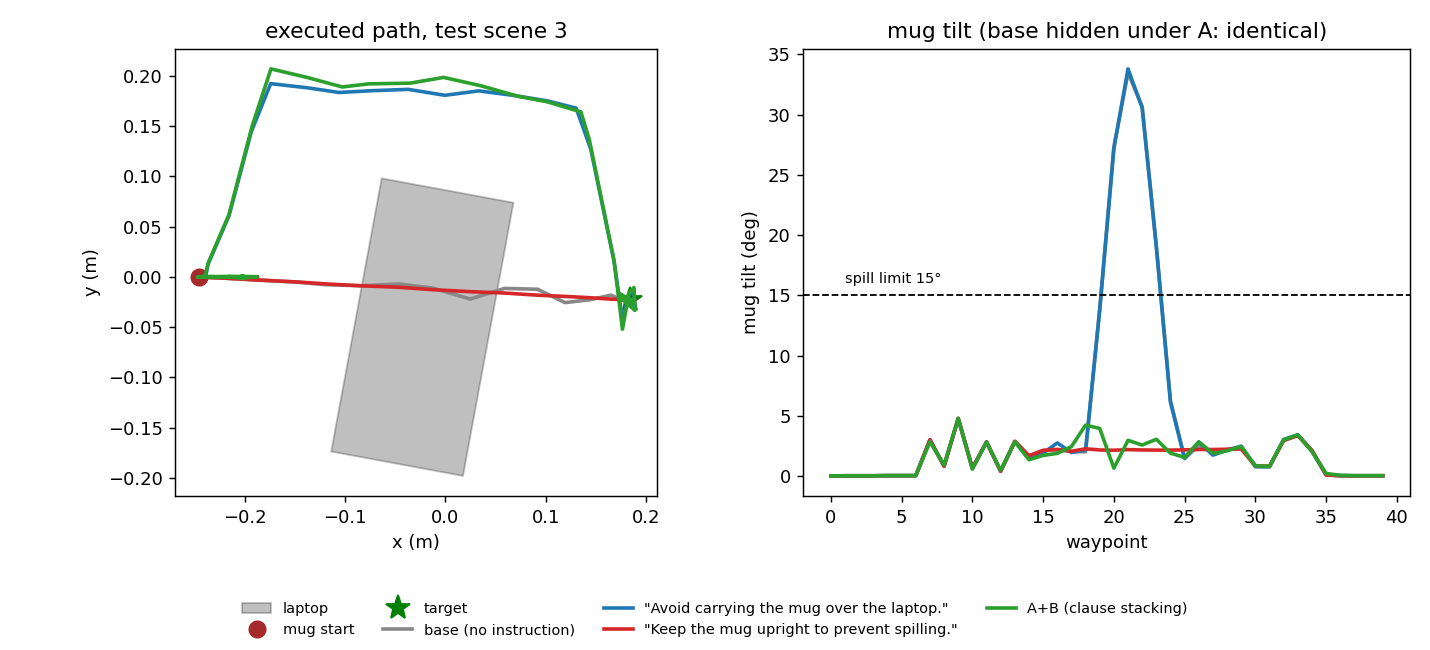
\includegraphics[width=0.95\linewidth]{figs/figure_scene.png}
\caption{Test scene 3, executed trajectories. The A instruction takes the mug around the laptop
and keeps the base tilt. The B instruction keeps the straight path and removes the tilt.
Applying the two clauses in turn does both.}
\label{fig:scene}
\end{figure}

%=====================================================================
\section{Experiment 1: swapping the instruction}

\paragraph{Where it works.} Everywhere we looked. With the scene and base trajectory held
fixed, the A text produces a detour averaging 5.9\,cm and no rotation change; the B text
produces a 5.6-degree orientation fix and no path change. The empty instruction returns the
base trajectory untouched. Task success stays at 99 to 100\% (Figure~\ref{fig:exp1}).

\begin{figure}[htbp]
\centering
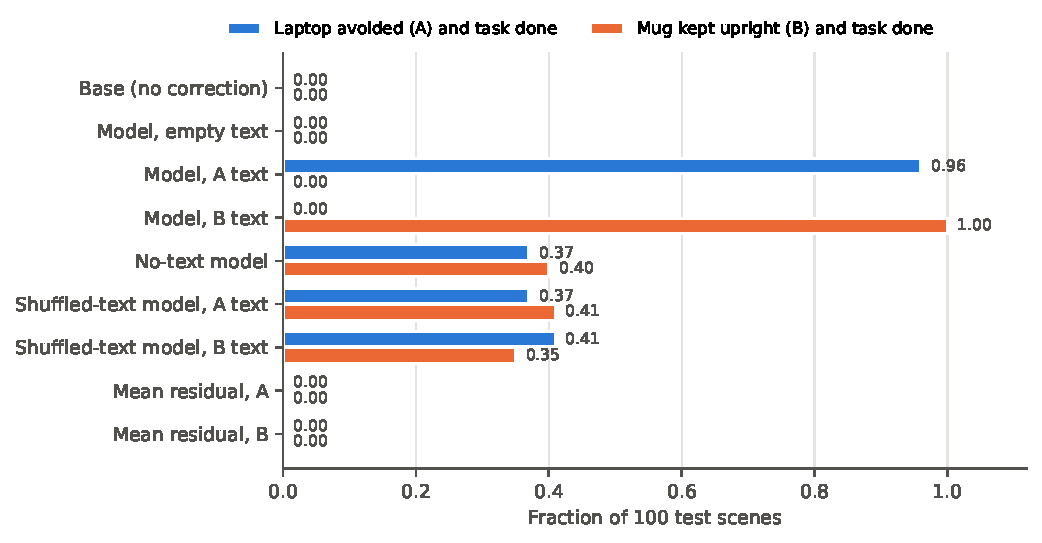
\includegraphics[width=0.9\linewidth]{figs/exp1_swap.pdf}
\caption{Experiment 1 on the 100 test scenes. Only the right instruction fixes each constraint.
Models without usable text land near 40\% on both, and the average correction per instruction
fixes nothing.}
\label{fig:exp1}
\end{figure}

\paragraph{The baselines.} The no-text and shuffled-text models score about 40\% on each
constraint, whatever the instruction. Without a usable signal they produce an A-like, B-like or
empty correction at random, in roughly the training proportions. The average correction per
instruction fixes 0\% of scenes. For A, the left and right detours cancel in the average. For B,
the tilt axis and timing change from scene to scene, so the average tilt fix is about 0.2
degrees. Every comparison against the main model gives $p<10^{-16}$ (paired by scene; for
example, A text against shuffled text: 58 scenes better, 0 worse).

\paragraph{Insight.} The model reads the scene as well as the text. Which side to detour on
depends on where the laptop sits, and the model chooses the same side as the reference on 93\%
of samples. A model that had memorized one correction per sentence would score 0\%, as the
average-correction baseline does.

%=====================================================================
\section{Experiment 2: unseen paraphrases}

We wrote 8 new phrasings for each constraint, including the two from the plan, and scored each on
the 100 test scenes (Figure~\ref{fig:exp2}).

\begin{figure}[htbp]
\centering
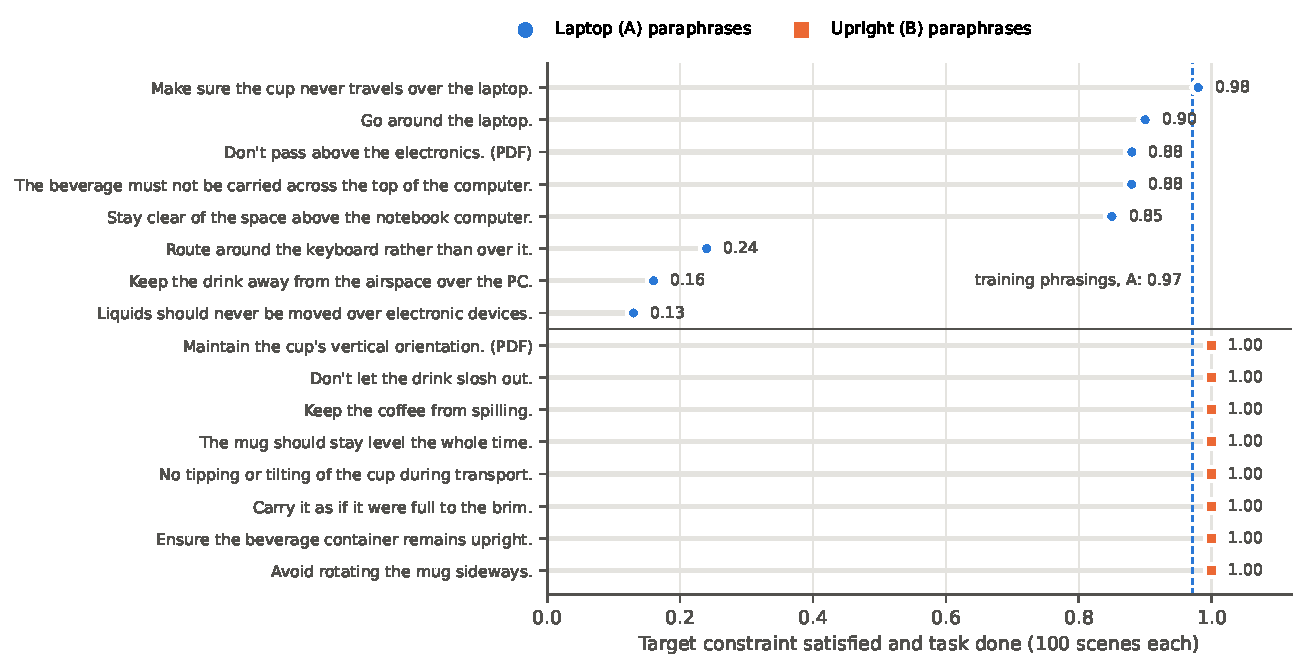
\includegraphics[width=0.95\linewidth]{figs/exp2_paraphrases.pdf}
\caption{Experiment 2. Every new upright phrasing works. Five of the eight new laptop phrasings
work, and three fail. The dashed line marks the score for the laptop training phrasings.}
\label{fig:exp2}
\end{figure}

\paragraph{Where it works.} All 8 upright phrasings score 100\%, including ``Maintain the cup's
vertical orientation'' and ``Carry it as if it were full to the brim.'' Five laptop phrasings
score 85 to 98\%, including the plan's ``Don't pass above the electronics'' at 88\%. In every
case the other constraint stays untouched and the task still succeeds 99 to 100\% of the time,
so the model never mistakes one constraint for the other on these phrasings.

\paragraph{Where it fails.} ``Route around the keyboard rather than over it'' (24\%), ``Keep the
drink away from the airspace over the PC'' (16\%), and ``Liquids should never be moved over
electronic devices'' (13\%). The model still detours for these, but by 3.6 to 4.0\,cm instead of
5.9\,cm, which is not enough to clear the laptop. Pooled over the 8 laptop phrasings, the score
is 63\%.

\paragraph{Insight.} Text similarity does not predict which phrasings fail. In BGE's embedding
space every held-out phrasing sits closer to its own constraint's training phrasings than to the
other's, so the encoder separates them correctly. The loss happens in the model's mapping from
embedding to correction: a phrasing that lands away from the five training points gets treated
as a partial mix of ``laptop'' and ``no instruction'', and the detour shrinks. The upright result
is also the easier one. Its correction just undoes the tilt already visible in the base
trajectory, while the laptop correction depends on the scene geometry.

\subsection*{Follow-up: mixing training embeddings}

We added one change after seeing these results. During training, each instruction embedding
became a random blend of two same-constraint training phrasings plus a little noise. Since we had
already seen the failing phrasings, we wrote a second, fresh set of 8 + 8 paraphrases before
training and scored on that set (Figure~\ref{fig:aug}).

\begin{figure}[htbp]
\centering
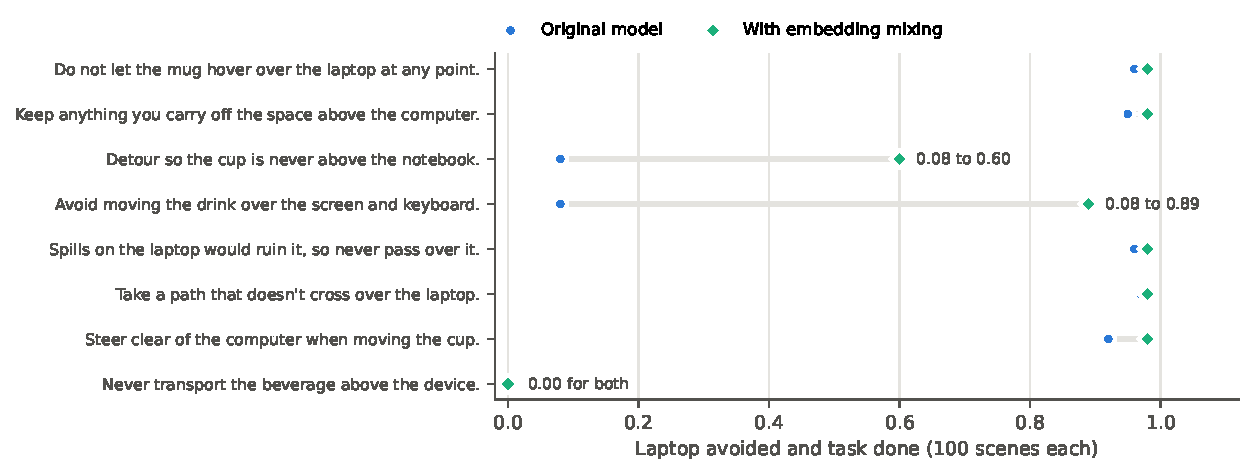
\includegraphics[width=0.95\linewidth]{figs/aug_heldout2.pdf}
\caption{Fresh laptop paraphrases, before and after embedding mixing. Two phrasings recover
sharply. One phrasing scores 0.00 for both models.}
\label{fig:aug}
\end{figure}

\begin{itemize}
  \item The original model scored 61.5\% on the fresh laptop set, almost the same as on the
        first set (61.9\%), so the first set was not unusually hard.
  \item With mixing, the fresh laptop set rose to 79.9\% [77.0, 82.5]. Paired by phrasing and
        scene, mixing was better 149 times and worse 2 times. Training phrasings and all upright
        phrasings were unchanged.
  \item The recovered phrasings now produce full-size detours (5.0 to 5.4\,cm, up from about
        3.3\,cm), which explains the gain.
  \item ``Never transport the beverage above the device'' fails in a different way. Both models
        read it as an upright instruction: they output a rotation fix and almost no detour.
        Mixing does not help with this kind of confusion between the two constraints.
  \item Each model was trained once, so we have not measured how much the gain varies with the
        training seed. Three seeds of each would settle it (about 30 GPU minutes).
\end{itemize}

%=====================================================================
\section{Experiment 3: the unseen combined instruction}
\label{sec:exp3}

We tested six combined sentences, such as ``Avoid carrying the mug over the laptop and keep the
mug upright to prevent spilling'' and ``Carry the mug around the laptop without tilting it.''
None appeared in training.

\paragraph{Where it fails.} Given the sentence directly, the model satisfied both constraints in
0 of 1{,}200 runs [0.0, 0.3\%]. It picks one constraint, or does a weak version of one, or does
neither. It never breaks the task (success stays at 100\%). The method the plan listed as an
option, adding the two instructions' flows at inference time, scored 3\%: it keeps part of the
tilt fix and loses most of the detour. That happened even when the two clauses were the exact
training sentences, so the problem is in how the flows combine, not in reading the text.

\begin{figure}[htbp]
\centering
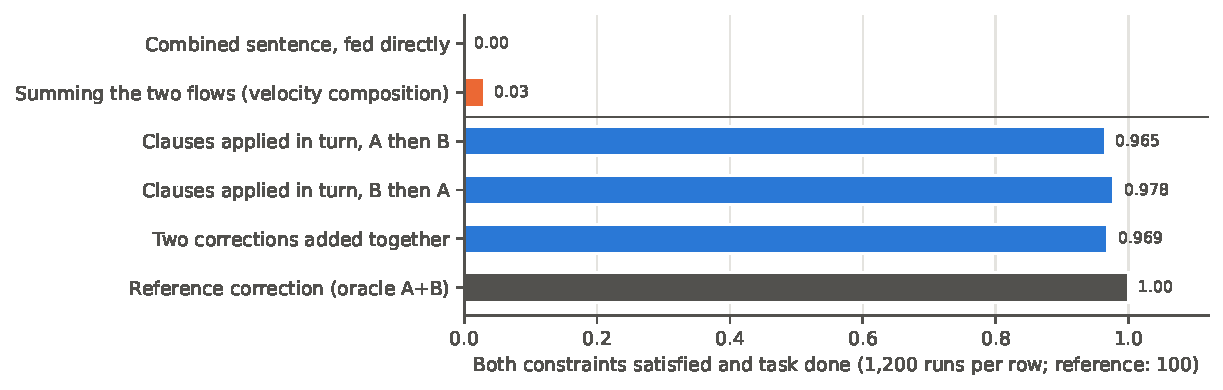
\includegraphics[width=0.9\linewidth]{figs/exp3_compose.pdf}
\caption{Experiment 3. Orange: the two methods that ask the model to combine inside one pass.
Blue: applying the learned corrections separately. Grey: the reference correction.}
\label{fig:exp3}
\end{figure}

\paragraph{Why it fails.} Every laptop training example keeps the tilt, and every upright
example keeps the straight path. A trajectory that both detours and stays upright is unlike
anything either instruction produced in training, so neither the combined sentence nor the sum
of the two flows has anywhere to go. The design choice that makes Experiment 1 clean (A must not
touch orientation, B must not touch the path) is the same one that blocks combining the two
inside one model pass.

\paragraph{Where it works.} We split each sentence into its two clauses by hand and applied the
corrections one after the other, with no retraining. The second correction runs on a trajectory
it never saw in training: in the B-then-A order, the laptop correction receives a tilt-free base,
and every training base was tilted at least 35 degrees. Both constraints were met with task
success on 96.5\% of runs in the A-then-B order and 97.8\% in the B-then-A order. Against the
direct sentence, this won on 89 to 100 of 100 scenes for every instruction and lost on none.

\paragraph{Insight.} Simply adding the two corrections scores 96.9\%, about the same as applying
them in turn. That is because A only changes the path and B only changes the orientation, so the
two fixes never interfere. The 97\% shows that each learned correction holds up on unfamiliar
base trajectories. It does not show that the model can reason about two constraints together.
Testing that needs constraints that interact, for example a detour that is only possible if the
mug is held at a particular angle.

%=====================================================================
\section{Insights}

\begin{enumerate}
  \item \textbf{Language controls the correction.} The instruction alone decides which
        constraint gets fixed, and the model adapts the fix to the scene. This is the core of the
        hypothesis, and it holds with large margins.
  \item \textbf{Generalizing to new wordings depends on the constraint.} When the correction
        mostly comes from the base trajectory (upright), any reasonable wording works. When it
        depends on scene geometry (laptop), wordings far from the training set produce a
        detour that is too small. Mixing training embeddings recovers most of the gap cheaply.
  \item \textbf{A frozen encoder is not the bottleneck.} BGE separates every held-out phrasing
        correctly. The errors come from the small learned mapping from embedding to correction,
        which only ever saw five points per constraint.
  \item \textbf{One sentence embedding does not combine constraints.} Neither the combined
        sentence nor summing flows works. Training on each constraint alone teaches the model
        that each correction must leave the other dimension untouched.
  \item \textbf{Separate corrections stack well.} Applied clause by clause, the learned
        corrections combine without retraining. An automatic clause splitter (a parser or a
        small language model) would make this usable.
\end{enumerate}

\section{Limitations}

\begin{itemize}
  \item The arm passes through objects; only the mug, laptop and table collide.
  \item The grasp is a rigid attachment, not finger contact. The mug collides as a box.
  \item ``Spill'' is a tilt above 15 degrees. There is no simulated liquid.
  \item The base policy is scripted, as the plan allows. A VLA would add noise and variety this
        setup does not have.
  \item A and B change separate parts of the action, which makes combining them easy once they
        are applied separately.
  \item Each model was trained with one seed. The Experiment 1 and Experiment 3 gaps are far
        larger than sampling noise; the embedding-mixing gain should be checked over seeds.
  \item Clauses were split by hand for the stacking follow-up.
\end{itemize}

\section{Next steps}

\begin{enumerate}
  \item Constraints that interact, so that combining them requires more than adding two
        independent fixes. This is the real test of Experiment 3.
  \item An automatic clause splitter in front of the stacking method.
  \item A three-seed rerun of the embedding-mixing comparison on the fresh paraphrase set.
  \item Replace the scripted base with a VLA policy in LIBERO.
\end{enumerate}

\vspace{1em}
\noindent\small Code and raw results: \texttt{experiments/residual\_flow\_poc/}
\\
\texttt{RESULTS.md} has every table, and \texttt{report/make\_report\_figs.py} draws these figures.

\end{document}
